\chapter{Results Analysis}

In this chapter, the results of all experiments are compared and discussed to evaluate which approach is suitable in which scenario. 

The experiments quickly showed that when trying to detect anomalies in time series with deep learning approaches, the described unsupervised approach is the preferred choice. As supervised approaches need to assure, that the anomalies that occur when the model is in operation are the same as in the training set. Further, in this case, a training set that contains a sufficient number of anomalies to train on must exist. Only under these limiting conditions a supervised model can reliably be deployed. When these requirements are fulfilled a Convolutional Neural Network might be a good choice. 
Experiment 1 showed that a CNN, in comparison to a RNN, is capable of recognizing the anomalies. The same conclusion was reached by Wen and Keyes \parencite*{Wen2019}, who successfully applied a special version of a CNN (U-Net: Section \ref{U-Net}) to the GHL dataset.  

In contrast to the supervised approach the unsupervised approach generally proved to be more stable. As it needs no knowledge of the nature of the anomalies. The only requirement for this approach is a sufficiently large training set to learn the normal behaviour. Both neural network types, CNN and RNN, showed similar abilities when learning the normal behaviour. This means that CNNs, that are usually applied for tasks such image recognition, are similarly suitable to predict time series, which is normally the domain of RNN. Looking at the F1-Scores of Experiments 1 to 3, shows that CNN can be a useful alternative to RNN when detecting anomalies. Although, the F1-Score of the CNN is often marginally lower than the F1-Score of the compared RNN, the CNN has another big advantage. When tracking anomalies, it is often a necessary to detect them as quickly as possible. Looking at the inference times of the various models, it can be seen that the CNN model is up to three times faster than the RNN model. This advantage of speed can be of paramount importance in a real-world scenario, as it can decide if delicate components of a system take damage or not.

The CNN is not only faster at inference but also in training. As there many hyper-parameters, such as batch size, lookback, layers etc., to be determined for an optimal model performance, the training time becomes important. When using a machine learning algorithm, a model is trained again and again to find the best configuration. So the training time of a model decides how fast a well performing model can be developed. Looking at the training times achieved in this work, it can be seen that the CNN learns much faster. This might have two reasons. First, when the number of parameters in the CNN and RNN models are compared, it can be observed, that a CNN generally has less parameters (see Appendix \ref{AppendixA}). When training a neural network, after every batch, it needs to be calculated, how much these parameters need to be adjusted. This makes it more and more computationally expensive the more parameters there are. Second, it seems to be good strategy to look at a time series as a pattern. Where the RNN calculated the influence of the past on the future, the CNN tries to recognise patterns in the data. This approach not only worked when the time series followed a cyclic pattern as Experiment 1 and 3 but also in the case of the weather data in Experiment 2.     

Ultimately, as it is often the case in data science, the choice whether to use RNN or CNN is a trade-off, in this particular case, between speed and quality of the result. This trade-off might be mitigated in the favour of the CNN, by using more advanced versions of the CNN such as the U-Net.


\section{Review of Experiments}
Neural Networks became popular in recent years in anomaly detection as they require little domain knowledge. The experiments conducted in this work indicate that this comes at the expense of higher training and inference times as well as performance drawbacks. This is particularly evident in Experiment 3. As Figure \ref{fig:review} shows, one type of anomaly is easily recognizable. The green line represents the actual value, the red line indicates the anomalies. An anomaly occurs when the green line surpasses the 333°C threshold represented by the black line. 

\begin{figure}[h]
	\centering
	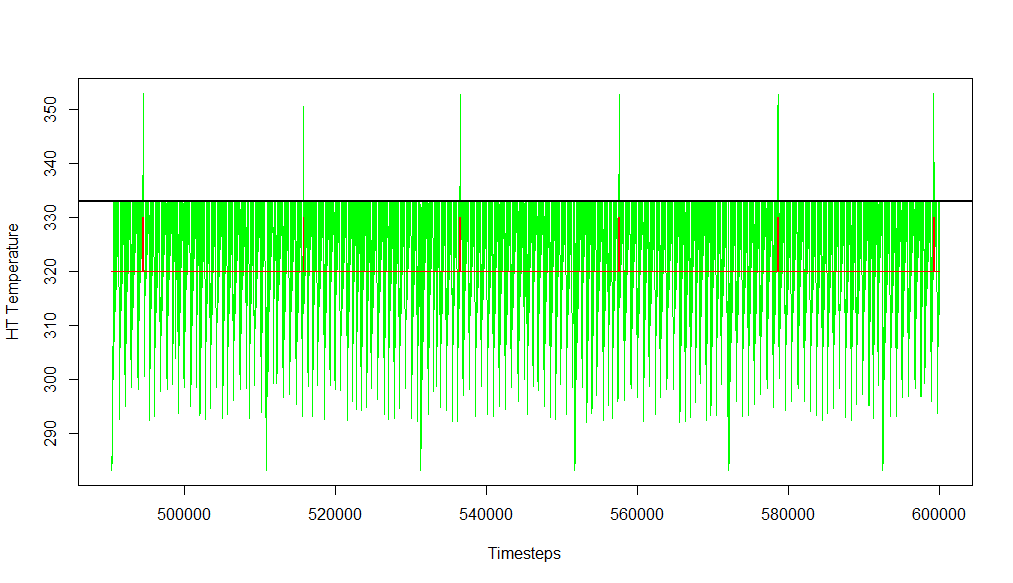
\includegraphics[scale=0.45]{Figures/review}
	\decoRule
	\caption[Behaviour of Anomaly in the GHL Dataset]{Behaviour of Anomaly in the GHL Dataset \parencite{own}}
	\label{fig:review}
\end{figure}

The above described anomalous behaviour is supposed to be known by someone with domain expertise. As a result, it is known that a Logistic Regression Model (see Appendix \ref{logitRegression}) is adequate for this type of anomaly, and that this much simpler model achieves 100 percent accuracy. 

Further, if the models of Experiments 1 and 3 were compared to the expected results of a Naïve Model (see Appendix \ref{naiveModel}), it is likely that the Naïve Model is at least as effective as the dataset, or at least on certain variables, as they follow predefined patterns. This good performance may be achieved by the Naïve Model because the complexities of the datasets of Experiments 1 and 3 are quite low. It is therefore advisable to thoroughly analyse a dataset before applying an anomaly detection method as a simple method may produce the best results.    

To conclude, deep learning is not always the best option, and domain expertise and a complete analysis of the dataset is still necessary to select a quick and accurate model. This statement is supported by Braei and Wagner's \parencite*{Braei2020} findings, which suggests that deep learning is most beneficial for contextual anomalies.   

\chapter{Conclusion}

This final chapter seeks to answer the research questions proposed in Section \ref{research_questions}. Further, the results of this work are discussed in regard to the thesis statement proposed in Section \ref{thesisstatement}

\section{Answering the Research Questions}


\paragraph{How does a CNN for univariate and multivariate data need to be designed for successful anomaly detection in time series data?}

Munir \parencite*{Munir2019} showed that for univariate time series data 1-dimensional convolutional layers can successfully be used. Wen and Keyes \parencite*{Wen2019} also use 1-dimensional convolutional layers for their proposed architecture type, the U-Net. The further design of the CNN for anomaly detection is dependent on the given task. If a supervised approach is deemed suitable, the CNN is used as a classifier deciding whether a given sequence is anomalous or not. However, this approach is reserved only for a few special use cases where the shapes of the anomalies are known and unchanging. If it is unknown how the anomalies look like, the CNN has to be designed to predict the future of a time series. Given this so-called regression task, it is preferable to omit the max-pooling layers, that are normally part of CNN architecture, because especially with complex multivariate time series, they impair a CNN's ability to reliably predict a time series.  

\paragraph{What advantages and disadvantages arise when using a CNN compared to a RNN for anomaly detection in univariate and multivariate time series?} The main advantage of a CNN over an RNN, such as a GRU- or LSTM-neural network, is its shorter computation time. The research revealed that utilizing a CNN reduces the amount of time it takes to train and infer. This is especially useful in the use case of anomaly detection as it is crucial to recognize the anomalies as fast as possible.

The second big advantage of a CNN is its ability to recognize anomalies. Given a case where the anomalous behaviour always follows the same pattern as in Experiment 1, a CNN can reliably be trained to recognize this pattern. A real world scenario for this use case be the frequency analysis of a ball bearing \parencite{Mais2002}. The frequency at which the ball bearing oscillates correlates with the expected remaining service life. A CNN can now be trained to recognize this pattern and reliably indicate, whether it needs to be replaced.

In the scope of this work no major disadvantages were found when comparing CNN to RNN to detect anomalies.


\paragraph{Which hyper-parameter settings are crucial for a fair performance comparison between RNN and CNN?} In order to fairly compare the two neural network architectures, whereever possible the hyperparameters were defined for both types. These hyperparameters include foremost the configuration of the generator function. Further, regarding the neural network architecture, the given task and the applied optimizer was defined the same for both types. At last, when postprocessing the data, that was produced by the experiments, parameters were set to the same value, for example how the rolling mean was calculated in Experiment 3.

In contrast, it is difficult to compare the neural network architectures, because the functionalities are fundamentally different. Even when the neural networks have the same number of layers and roughly the same number of neurons, as in Experiment 2, the number of trainable parameters is vastly different (see Appendix \ref{exp2_summary}). During the experiments conducted in this work, the hyperparameters defining the neural networks were set on an experimental basis. No hyperparameter-tuning routine was used, with the disadvantage of probably suboptimal results, but with the advantage of being able to build neural networks with similar complexity. Except for Experiment 3, the neural networks were designed with the same number of layers and approximately the same number of neurons.

\textcolor{red}{ Interestingly, this approach showed, that the learning capabilities of the neural networks were similar.}

\section{Insights Regarding Thesis Statement}

\textbf{Convolutional Neural Networks are superior to Recurrent Neural Networks when looking for anomalies in time series data regarding training time and complexity.}\\
\\
The experiments conducted in this work did not show that Convolutional Neural Networks are overall superior to Recurrent Neural Networks. They have, nevertheless, been proved to offer significant benefits, particularly in the context of anomaly detection. The biggest advantage of CNN, is the reduced computation time, which helps to faster identify anomalies. The shorter computation time further becomes important once the experiment is scaled to bigger datasets and faster GPU aided hardware. At a certain complexity, the cost to run such deep learning based models will become incisive. Since deep learning is also sometimes criticised to not be eco-friendly, CNN offer an approach to mitigate both of these problems \parencite{Walleser2021}.

The trials conducted in this paper revealed that when a typical CNN with convolutional and max-pooling layers is applied, the performance is still inferior to that of an RNN. This gap, however, migth be closed, with the use of upsampling and transposing layers \parencite{Wen2019}. These, also called deconvolutional layers, build the counterpart to convolutional layers. Simply said convolutional layers' goal is to extract features, whereas deconvolutional layers' goal is to produce features. Wen and Keyes \parencite*{Wen2019} were able to successfully use the combination of both, convolution and deconvolution, in their anomaly detection experiment.

Overall, the experiments demonstrated that CNNs are capable of accurately forecasting time series. With some adjustments, they are probably equally as accurate as RNN. This work supports the view of some experts who believe RNN will be phased out in the future \parencite{Culurciello2018} \parencite{Bai2018}. 

% Some argue that RNN are no longer needed https://www.macnica.co.jp/business/ai_iot/columns/135112/
%https://towardsdatascience.com/the-fall-of-rnn-lstm-2d1594c74ce0
%https://arxiv.org/abs/1803.01271
\clearpage
\section{Future Research}
Through the work on this thesis, various areas of future research have been identified.

First, since it has been established that CNNs are useful for predicting time series, it should be investigated what configuration of CNN is best suited for this purpose. Potential architectures that could be capable of exceeding the accuracy of LSTMs include the autoencoder architecture (see \ref{U-Net}), the U-Net presented by Wen and Keyes \parencite*{Wen2019} or the Fully Convolutional Neural Network (FCN) first proposed by Wang \parencite*{Wang2017}.

Further, Verner \parencite*{Verner2019} and Braei and Wagner \parencite*{Braei2020} did comprehensive studies on what approaches are useful for anomaly detection. They compared methods such as Random Forrests or Clustering against deep learning approaches to find the anomalies. Only Braei and Wagner \parencite*{Braei2020} included CNN in their work on univariate anomalies. The experiments conducted in the scope of this paper showed that CNN achieve a similar performance on multivariate datasets to LSTM. It is thus suggested that more comprehensive studies are done with different datasets. As Wu and Keogh \parencite*{Wu2020} showed, some datasets are flawed, therefore, possible biases towards certain methods can arise, as in total only 3 different datasets have been used by the above mentioned studies. Another study on various multivariate datasets including CNNs would complement the overall picture of which anomaly detection methods are useful for which use cases.


% Verner used one dataset 
% Braei and Wagner used two
% potential for bias reliable and complete information needed looking at critics of Wu and Keogh





